% Font options: 10pm, 11pt, 12pt
% Align headings left instead of center: nocenter
\documentclass[xcolor=x11names,compress]{beamer}\usepackage[]{graphicx}\usepackage[]{color}
% maxwidth is the original width if it is less than linewidth
% otherwise use linewidth (to make sure the graphics do not exceed the margin)
\makeatletter
\def\maxwidth{ %
  \ifdim\Gin@nat@width>\linewidth
    \linewidth
  \else
    \Gin@nat@width
  \fi
}
\makeatother

\definecolor{fgcolor}{rgb}{0.345, 0.345, 0.345}
\newcommand{\hlnum}[1]{\textcolor[rgb]{0.686,0.059,0.569}{#1}}%
\newcommand{\hlstr}[1]{\textcolor[rgb]{0.192,0.494,0.8}{#1}}%
\newcommand{\hlcom}[1]{\textcolor[rgb]{0.678,0.584,0.686}{\textit{#1}}}%
\newcommand{\hlopt}[1]{\textcolor[rgb]{0,0,0}{#1}}%
\newcommand{\hlstd}[1]{\textcolor[rgb]{0.345,0.345,0.345}{#1}}%
\newcommand{\hlkwa}[1]{\textcolor[rgb]{0.161,0.373,0.58}{\textbf{#1}}}%
\newcommand{\hlkwb}[1]{\textcolor[rgb]{0.69,0.353,0.396}{#1}}%
\newcommand{\hlkwc}[1]{\textcolor[rgb]{0.333,0.667,0.333}{#1}}%
\newcommand{\hlkwd}[1]{\textcolor[rgb]{0.737,0.353,0.396}{\textbf{#1}}}%
\let\hlipl\hlkwb

\usepackage{framed}
\makeatletter
\newenvironment{kframe}{%
 \def\at@end@of@kframe{}%
 \ifinner\ifhmode%
  \def\at@end@of@kframe{\end{minipage}}%
  \begin{minipage}{\columnwidth}%
 \fi\fi%
 \def\FrameCommand##1{\hskip\@totalleftmargin \hskip-\fboxsep
 \colorbox{shadecolor}{##1}\hskip-\fboxsep
     % There is no \\@totalrightmargin, so:
     \hskip-\linewidth \hskip-\@totalleftmargin \hskip\columnwidth}%
 \MakeFramed {\advance\hsize-\width
   \@totalleftmargin\z@ \linewidth\hsize
   \@setminipage}}%
 {\par\unskip\endMakeFramed%
 \at@end@of@kframe}
\makeatother

\definecolor{shadecolor}{rgb}{.97, .97, .97}
\definecolor{messagecolor}{rgb}{0, 0, 0}
\definecolor{warningcolor}{rgb}{1, 0, 1}
\definecolor{errorcolor}{rgb}{1, 0, 0}
\newenvironment{knitrout}{}{} % an empty environment to be redefined in TeX

\usepackage{alltt}
%\documentclass[xcolor=x11names,compress,handout]{beamer}
\usepackage[]{graphicx}
\usepackage[]{color}
\usepackage{booktabs}
\usepackage{hyperref}
\usepackage{tikz}
\usepackage{multirow}
\usepackage{dcolumn}
\usepackage{bigstrut}
\usepackage{amsmath} 
\usepackage{xcolor,colortbl}
\usepackage{amssymb}
\usepackage{multicol}
%\newcommand{\done}{\cellcolor{teal}#1}

%% Beamer Layout %%%%%%%%%%%%%%%%%%%%%%%%%%%%%%%%%%
\useoutertheme[subsection=false,shadow]{miniframes}
\useinnertheme{default}
\usefonttheme{serif}
\usepackage{Arev}
\usepackage{pdfpages}

\setbeamerfont{title like}{shape=\scshape}
\setbeamerfont{frametitle}{shape=\scshape, size=\normalsize}

\definecolor{dkblue}{RGB}{0,0,102}

\setbeamercolor*{lower separation line head}{bg=dkblue} 
\setbeamercolor*{normal text}{fg=black,bg=white} 
\setbeamercolor*{alerted text}{fg=red} 
\setbeamercolor*{example text}{fg=black} 
\setbeamercolor*{structure}{fg=black} 
 
\setbeamercolor*{palette tertiary}{fg=black,bg=black!10} 
\setbeamercolor*{palette quaternary}{fg=black,bg=black!10} 

\renewcommand{\(}{\begin{columns}}
\renewcommand{\)}{\end{columns}}
\newcommand{\<}[1]{\begin{column}{#1}}
\renewcommand{\>}{\end{column}}

\AtBeginSection{\frame{\sectionpage}}
\usepackage{xcolor}
\hypersetup{
    colorlinks,
    linkcolor={red!50!black},
    citecolor={blue!50!black},
    urlcolor={blue!80!black}
}

\setbeamertemplate{navigation symbols}{} 
\setbeamertemplate{footline}[frame number]
\setbeamertemplate{caption}{\raggedright\insertcaption\par}

\setbeamersize{text margin left=5pt,text margin right=5pt}

%%%%%%%%%%%%%%%%%%%%%%%%%%%%%%%%%%%%%%%%%%%%%%%%%%


\title{FLS 6441 - Methods III: Explanation and Causation}
\subtitle{Week 12 - Review \& Frontiers}
\author{Jonathan Phillips}
\date{May 2020}
\IfFileExists{upquote.sty}{\usepackage{upquote}}{}
\begin{document}




\frame{\titlepage}

\section{Review}

\begin{frame}
\frametitle{Classification of Research Designs}
\begin{itemize}
\item Correlation is not causation
\begin{itemize}
\item And regresssion is just fancy correlation
\end{itemize}
\item So how do we provide evidence of causation?
\end{itemize}
\end{frame}

\begin{frame}
\frametitle{Classification of Research Designs}
\footnotesize
\begin{table}[htbp]
  \centering
  \scalebox{0.7}{
    \begin{tabular}{|p{2.2cm}|p{5cm}|c|c|}
    \hline
          &       & \multicolumn{1}{p{2.4cm}|}{\textbf{Independence of Treatment Assignment}} & \multicolumn{1}{p{3cm}|}{\textbf{Researcher Controls Treatment Assignment?}} \bigstrut\\
    \hline
    \multicolumn{1}{|p{2.9cm}|}{\multirow{2}[4]{2.9cm}{\textbf{Controlled Experiments}}} & Field Experiments & \checkmark      & \checkmark  \bigstrut\\
\cline{2-4}          & Survey and Lab Experiments &  \checkmark     & \checkmark \bigstrut\\
    \hline
          &       &       &  \bigstrut\\
    \hline
    \multicolumn{1}{|p{2.9cm}|}{\multirow{3}[6]{2.9cm}{\textbf{Natural Experiments}}} & Natural Experiments &  \checkmark     &  \bigstrut\\
\cline{2-4}          & Instrumental Variables & \checkmark      &  \bigstrut\\
\cline{2-4}          & Discontinuities & \checkmark      &  \bigstrut\\
    \hline
          &       &       &  \bigstrut\\
    \hline
    \multicolumn{1}{|p{2.9cm}|}{\multirow{4}[8]{2.9cm}{\textbf{Observational Studies}}} & Difference-in-Differences &       &  \bigstrut\\
\cline{2-4}          & Controlling for Confounding &       &  \bigstrut\\
\cline{2-4}          & Matching &       &  \bigstrut\\
\cline{2-4}          & Comparative Cases and Process Tracing &       &  \bigstrut\\
    \hline
    \end{tabular}}%
  \label{tab:addlabel}%
\end{table}%
\normalsize
\end{frame}

\begin{frame}
\frametitle{Definitions}
\begin{multicols}{2}
\begin{enumerate}
\item Potential Outcomes
\pause
\item Treatment Assignment Mechanism
\pause
\item Independence of Potential Outcomes from Treatment
\pause
\item Average Treatment Effect
\pause
\item Local Average Treatment Effect
\pause
\item Non-compliance
\pause
\columnbreak
\item Hawthorne Effects
\pause
\item Time-invariant confounder
\pause
\item Exclusion Restriction
\pause
\item Back-door path
\pause
\item SUTVA
\pause
\item Overlap in sample characteristics
\end{enumerate}
\end{multicols}
\end{frame}

\begin{frame}
\frametitle{Choosing a Method}
\begin{knitrout}
\definecolor{shadecolor}{rgb}{0.969, 0.969, 0.969}\color{fgcolor}
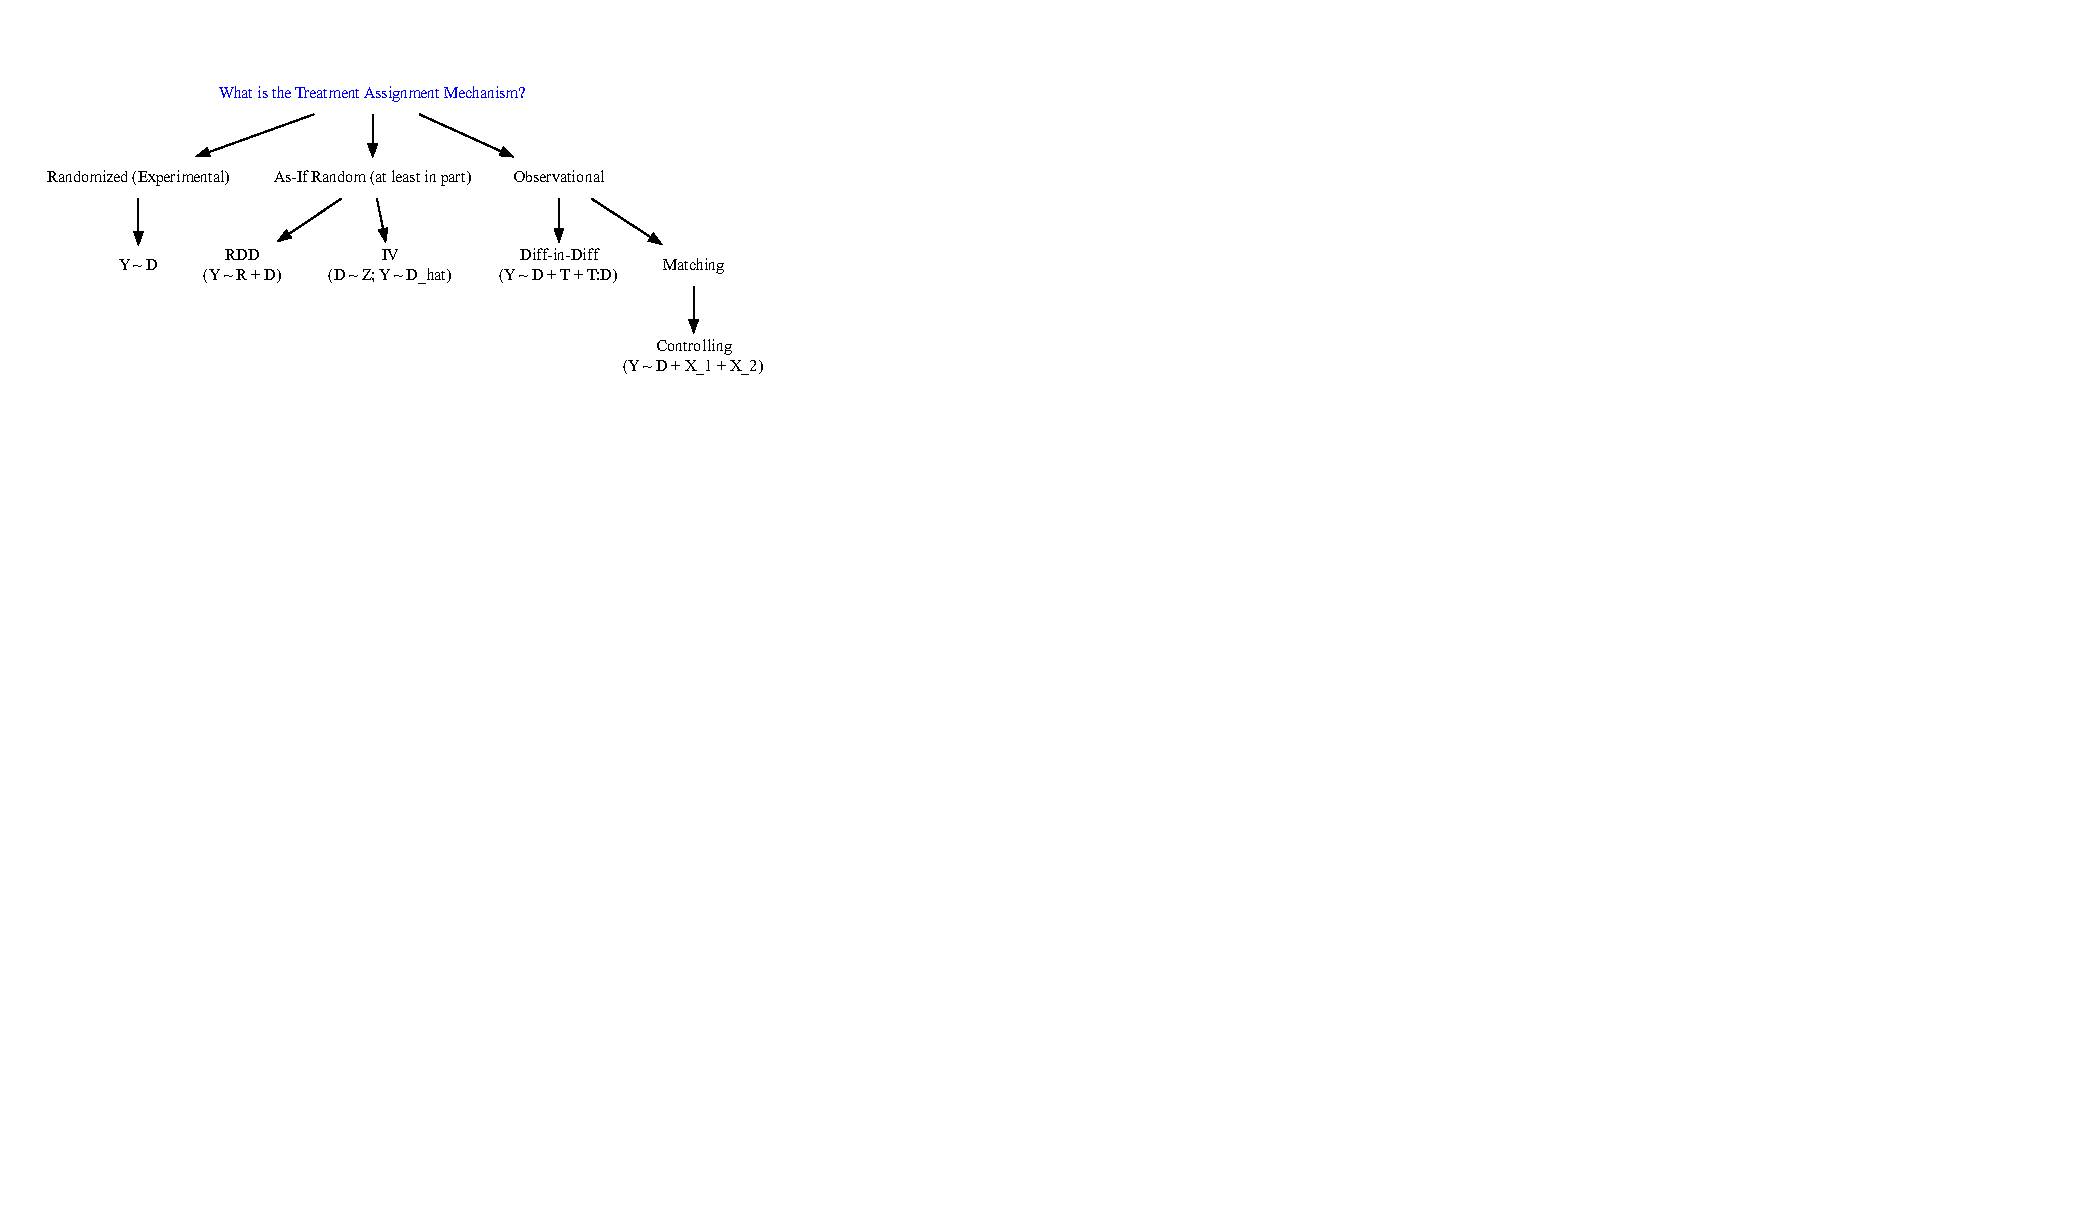
\includegraphics[width=2.7\linewidth]{figure/Dag1-1} 

\end{knitrout}
\end{frame}

\begin{frame}
\frametitle{Choosing a Method}
\begin{itemize}
\item How do we decide which causal inference strategy to use?
\pause
\begin{enumerate}
\item What is the treatment assignment mechanism?
\pause
\begin{itemize}
\item Randomized: field experiment
\item As-if random: natural experiment
\item Messy: Observational study
\pause
\end{itemize}
\item Where is the (as-if random) variation in treatment statuss?
\pause
\begin{itemize}
\item At discontinuous threshold: RDD
\item Before treatment: IV 
\item Across time and units: Diff-in-diff
\item Across units: Matching/Controls/Comparative case studies
\item None: Process Tracing
\end{itemize}
\pause
\item How many units can we get accurate measures for?
\pause
\begin{itemize}
\item One: Process tracing
\item Small-N: Comparative Case Studies
\item Large-N: Controls/Matching
\end{itemize}
\pause
\item Are the assumptions met?
\pause
\begin{itemize}
\item Parallel trends, no sorting, balance...
\end{itemize}
\end{enumerate}
\end{itemize}
\end{frame}

\begin{frame}
\frametitle{Choosing a Method}
\begin{enumerate}
\item Has experience with Obamacare increased electoral turnout?
\pause
\begin{itemize}
\item Difference-in-differences between states that did/did not expand Obamacare
\pause
\end{itemize}
\item Can playing a video game as a Roma character reduce anti-Roma prejudice in Hungary?
\pause
\begin{itemize}
\item Online survey experiment
\pause
\end{itemize}
\item Does peasant revolt in 19th century Russia lead to less representative local government?
\pause
\begin{itemize}
\item Instrument peasant revolt with serfdom
\pause
\end{itemize}
\item Do women govern differently from men? 
\pause
\begin{itemize}
\item Regression discontinuity in close elections in Brazil
\pause
\end{itemize}
\item Do US political contact campaigns change voters' choices?
\pause
\begin{itemize}
\item Field experiment
\pause
\end{itemize}
\end{enumerate}
\end{frame}

\begin{frame}
\frametitle{The Role of Theory}
\begin{itemize}
\item Political Scientists test \textbf{theories}, not interventions
\pause
\item To avoid \textbf{data mining} and multiple testing: We have to test plausible, relevant and falsifiable theories
\pause
\item To tell us \textbf{which experiments} and research designs to run
\pause
\item To \textbf{justify assumptions} (exclusion restriction, confounders)
\pause
\item To help us \textbf{interpret} what we have learned
\end{itemize}
\end{frame}

\begin{frame}
\frametitle{The Role of Qualitative Evidence}
\begin{itemize}
\item Vital for 'finding' natural experiments
\pause
\item To \textbf{validate assumptions} (no sorting, randomization worked, SUTVA)
\pause
\item To understand specific \textbf{analysis requirements}, eg. non-compliance, clustering
\pause
\item For Process Tracing: \textbf{Causal Process Observations}
\end{itemize}
\end{frame}

\begin{frame}
\frametitle{Comparing Methodologies}
\begin{itemize}
\item Different methodologies measure \textit{different treatment effects} for \textit{different populations}
\pause
\item Often a trade-off between \textbf{Bias} and \textbf{Generalizability}
\end{itemize}
\pause
\begin{multicols}{2}
\begin{itemize}
\item \textbf{Regression Discontinuity:}
\pause
\item Low bias, Low generalizability
\pause
\item LATE, estimated for a population where discontinuities were available
\end{itemize}
\columnbreak
\begin{itemize}
\item \textbf{Regression with Controls:}
\pause
\item High bias, High generalizability
\pause
\item ATE, estimated for the whole population we have data for
\pause
\item \textit{But}: Aronow and Samii (2016) - simple regression also implicitly weights your sample, so it's not as generalizable as you think
\end{itemize}
\end{multicols}
\begin{itemize}
\item We can do both and compare!
\end{itemize}
\end{frame}

\begin{frame}
\frametitle{Limitations of Causal Methodologies}
\begin{itemize}
\item Sure, you have shown that $D$ affects $Y$, but \textit{how}?? The connection is still a black box!
\pause
\item Causal effects are probably highly heterogeneous - do we really \textit{care about the ATE} (the average effect)?
\pause
\item They only tell us about \textit{'unusual'} parts of the population (eg. RDD, Field Experiment)
\pause
\item Even if variable X has a causal effect, \textit{how much} of the real world does it explain?
\pause
\item Sometimes it's just not possible to show causation. That's OK!
\begin{itemize}
\item We just need to recognize the limits of the evidence we have
\end{itemize}
\end{itemize}
\end{frame}

\section{Frontiers}

\begin{frame}
\frametitle{Frontiers of Strengthening Causal Arguments}
\begin{itemize}
\item Writing a paper means sustaining a convincing argument
\pause
\item Choosing and implementing an appropriate method is only the first step
\pause
\item We also need to show that our estimate is reliable and not a 'chance' finding
\pause
\item More importantly, that it is evidence in support of a \textbf{specific} theory
\pause
\item You don't want to publish a paper that someone contradicts next week!
\end{itemize}
\end{frame}

\begin{frame}
\frametitle{Robustness Tests}
\begin{itemize}
\item In general, we will trust our estimate more if it doesn't change even when we change our model
\pause
\begin{itemize}
\item Not just direction and significance, but in the substantive effect size
\pause
\end{itemize}
\item Alternative covariates/matching procedures
\pause
\item Alternative bandwidths/functional forms
\pause
\item Alternative (but conceptually equivalent) measures of key variables
\pause
\item Alternative samples (dropping outliers, different countries etc.)
\pause
\item Multiple tests of different parts of theory
\end{itemize}
\end{frame}

\begin{frame}
\frametitle{Sensitivity Analysis}
\begin{itemize}
\item An alternative is to ask - quantitatively - \textit{how much} do our results change when we alter the model or its assumptions?
\pause
\item One example for observational studies:
\begin{itemize}
\item How much larger would \textbf{unmeasured} confounders have to be than \textbf{measured confounders} to remove the entire estimated treatment effect? (Altonji et al 2005)
\pause
\end{itemize}
\item Eg. Nunn and Wantchekon (2011) argue that for unmeasured confounders to explain their estimated effect of the slave trade on trust, they would have to be 3 - 11 times larger than measured confounders
\end{itemize}
\end{frame}

\begin{frame}
\frametitle{Heterogeneity Tests}
\begin{itemize}
\item We have an average treatment effect
\pause
\item But theory may predict different groups are affected to different degrees
\pause
\item We can test for heterogeneous effects: \textbf{Conditional Average Treatment Effects (CATE)}
\pause
\item $Y_i \sim \beta_1 D_i + \beta_2 X_i + \beta_3 D_i*X_i + \epsilon_i$
\pause
\item $X_i$ MUST be a \textbf{pre-treatment} covariate we are testing for heterogeneous effects on
\pause
\item CRUCIAL: Our \textbf{covariate} is not randomly assigned, so the interpretation of heterogeneous effects is \textbf{not causal}, just descriptive
\end{itemize}
\end{frame}

\begin{frame}
\frametitle{Heterogeneity Tests}
\begin{itemize}
\item Ex. Ferraz and Finan (2008)
\begin{itemize}
\item Audits reduce corruption, they argue due to electoral accountability
\pause
\item The effects should therefore be stronger where:
\pause
\begin{itemize}
\item More people know about the audits (local radio): It is!
\pause
\item And for first-term Mayors with re-election incentives. It is!
\pause
\end{itemize}
\item Are there other theories consistent with \textit{all} of this evidence?
\pause
\item Note this does not mean that being a first-term mayor \textit{causes} audits to be more effective
\end{itemize}
\end{itemize}
\end{frame}

\begin{frame}
\frametitle{Heterogeneity Tests}
\begin{itemize}
\item But what if we look for heterogeneous effects on 20 variables?
\pause
\begin{itemize}
\item And then construct a theory to 'explain' the variables that show differential effects
\end{itemize}
\pause
\item Theory first! Avoid \textit{ex post} construction of theory and data-mining
\pause
\item At least correct p-values for multiple testing 
\pause
\item More details on this \href{https://egap.org/methods-guides/10-things-heterogeneous-treatment-effects}{egap page}
\end{itemize}
\end{frame}

\begin{frame}
\frametitle{Placebo Tests}
\begin{itemize}
\item How likely is it that our treatment effect is just a product of messy data?
\pause
\item Normally we test for a treatment effect where we \textbf{expect} one
\pause
\item But we can also test for a treatment effect where we \textbf{don't} expect one
\begin{itemize}
\item Evidence of \textbf{no} treatment effect supports our interpretation
\pause
\item Evidence of a 'surprising' treatment effect suggests messy data, or an incomplete theory
\end{itemize}
\pause
\item Common for regression discontinuities (alternative thresholds) and difference-in-differences (alternative times of treatment)
\end{itemize}
\end{frame}

\begin{frame}
\includegraphics[scale=0.4]{placebo_2.png}
\end{frame}

\begin{frame}
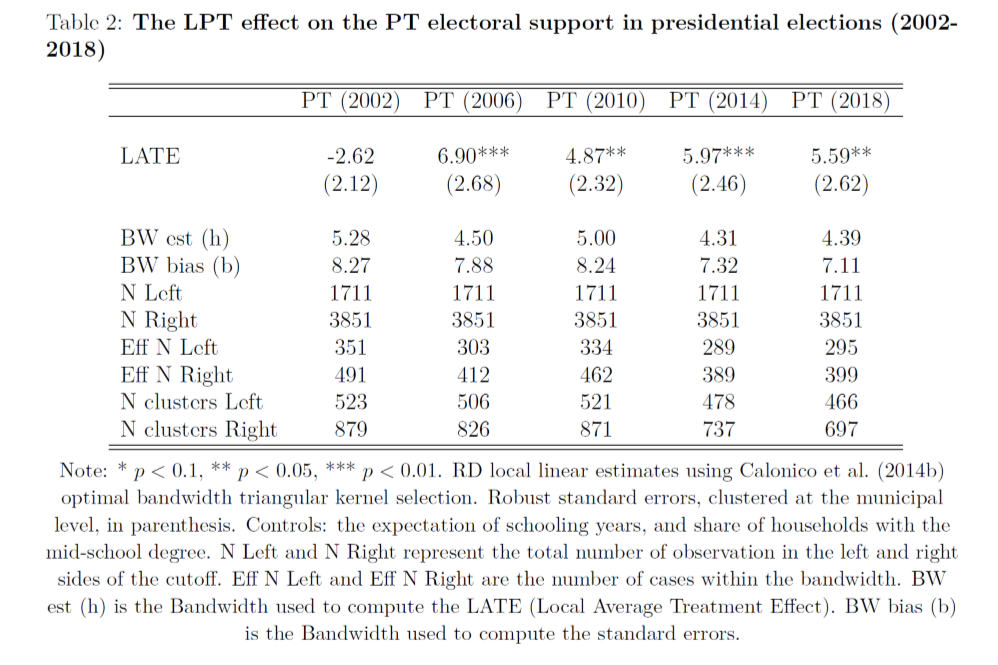
\includegraphics[width=\linewidth]{placebo.png}
\end{frame}

\begin{frame}
\frametitle{Generalizability}
\begin{itemize}
\item How 'weird' are the units we are measuring the Local Average Treatment Effect for?
\pause
\item We can try to \textit{describe} the characteristics of these compliers
\pause
\item We don't know if any single individual is a complier
\pause
\item But we can describe them \textbf{on average}
\pause
\item The first stage of the IV regression tells us about compliance with treatment
\pause
\item Relative likelihood that a complier has covariate X equals:
\end{itemize}
\pause
$$\frac{Pr(Complier | X_i=1)}{Pr(Complier)}$$
\end{frame}

\begin{frame}
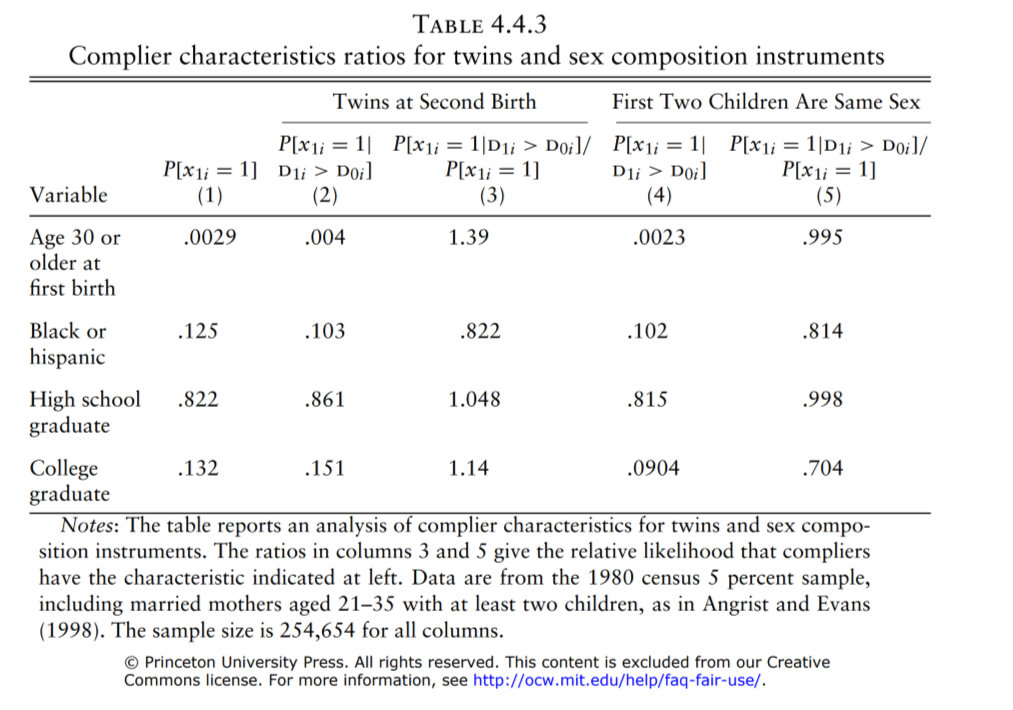
\includegraphics[width=\linewidth]{twins_compliers.png}
\end{frame}

\begin{frame}
\frametitle{Generalizability}
\begin{itemize}
\item Replication is crucial to our ability to generalize
\pause
\begin{itemize}
\item Replication in different samples from the same population
\pause
\item Replication in different populations
\pause
\item Replication of different treatment implementations
\end{itemize}
\pause
\item This is how we accumulate knowledge
\end{itemize}
\end{frame}

\begin{frame}
\frametitle{Mechanisms}
\begin{itemize}
\item To avoid the critique that experiments are a black box, and to support specific theories, we need to start testing \textbf{causal mechanisms}
\pause
\item We have already seen how to use process tracing to 'test' specific mechanisms in individual cases
\pause
\item Quantitative tests also exist, exploiting 'post-treatment bias'
\pause
\item But require additional assumptions: \textbf{Sequential ignorability}
\begin{itemize}
\item That the treatment is independent of potential outcomes
\pause
\item \textbf{AND} that the mediator (mechanism) is independent of potential outcomes conditional on treatment
\pause
\item Hard!
\end{itemize}
\end{itemize}
\end{frame}

\begin{frame}
\frametitle{Mechanisms}
\begin{itemize}
\item One practical approach is to run two regressions that recreates our DAG:
\end{itemize}
$$M_i = \alpha_1 + \beta_1 D_i + \epsilon_1$$ \\
$$Y_i = \alpha_3 + \beta_3 D_i + \beta_4 M_i + \epsilon_3$$ \\
\begin{itemize}
\item This implies:
\end{itemize}
$$Y_i = \alpha_3 + D_i (\beta_3+\beta_4*\beta_1) + (\alpha_1 +\epsilon_1)*\beta_4 + \epsilon_3$$
\pause
\begin{itemize}
\item Direct effect of treatment = $\beta_3$
\pause
\item Indirect effect of treatment = $\beta_4*\beta_1$
\end{itemize}
\end{frame}

\begin{frame}
\frametitle{Pre-Analysis Plans}
\begin{itemize}
\item There are a lot of tests and specifications we can run!
\pause
\item How do we know what is \textit{ex post} data-mining and what is a real test of a specific theory?
\pause
\item We can \textbf{constrain ourselves}
\pause
\item Submit a Pre-Analysis Plan, eg. to \href{https://egap.org/content/registration}{egap} or see \href{https://www.bitss.org/resource-tag/pre-analysis-plans/}{BITSS}
\pause
\item Document the theory and hypotheses you're using (to avoid fitting an explanation to the data)
\pause
\item Document the regressions you will run (to avoid data-mining)
\pause
\item If you need to change later, no problem! We just need to justify why
\pause
\item It's transparent how far away we have come from the original test of theory
\end{itemize}
\end{frame}


\end{document}
